\documentclass[11pt,oneside,openany,a4paper,%..... Layout
               afrikaans, english%.............. Global language selection
               ]{memoir}

 \usepackage[masters-t,%.......................... Master thesis
             goldenblock,%........................ A5 type block (or a5block or wide)
            ]{usthesis}%.......................... US thesis style with memoir

%
% PLEASE read the USthesis documentation for the class options
% and how to set line and paragraph spacing
%
%==== Language setup ================================================
 \usepackage[latin1]{inputenc}%................... Recognizes �, �, etc
 \usepackage{babel}%.............................. Language setup

%==== Math setup ====================================================
 \usepackage{amsmath}%............................ Advanced math (before fonts)
 \usepackage{amssymb}%............................ AMS Symbol fonts

%==== Font setup (default is Computer Modern) =======================
 \usepackage[T1]{fontenc}%........................ Type 1 fonts
 \usepackage{textcomp}%........................... Additional text character
 \usepackage{bm}%................................. Bold math symbols (after fonts)

%==== Ref's, Bib's and Nomencl ======================================
 \usepackage{usnomencl}%.......................... List of symbols (in usthesis pack)
 %\usepackage{usbib}%.............................. Bibliography    (in usthesis pack)
%    \bibliographystyle{usmeg-n}
%    \renewcommand\bibfont{\small}

    %% For usmeg-a, the bib is a list of references. If you
    %% are using usmeg-n comment out the following lines
    %\addto{\captionsafrikaans}{\renewcommand{\bibname}{Lys van Verwysings}}
    %\addto{\captionsenglish}{\renewcommand{\bibname}{List of References}}

%==== Graphics and Color ============================================
\usepackage{graphicx}%........................... Graphicx loaded in usthesis
\usepackage{color}%.............................. Color setup
\usepackage{eso-pic}%............................ Shipout commands for watermark
    \newcommand*{\WaterMark}[2][0.2\paperwidth]{%
        \AddToShipoutPicture*{\AtTextCenter{%
                \parbox[c]{0pt}{\makebox[0pt][c]{%
                    \includegraphics[width=#1]{#2}}}}}}

%==== Local Defs ====================================================
\makeatletter

%
% Please insert user defined commands here
% and NOT in the document itself!
%
%\usepackage{hyperref}
\usepackage[caption=false]{subfig}
\usepackage{sistyle}
    \SIstyle{S-Africa}
    \SIunitspace{{\cdot}}
    \SIunitdot{{\cdot}}
    
\renewcommand{\UScaptionsafrikaans}{%
    \def\DeclarationName{Verklaring}%
    \def\AbstractName   {Samevatting}%
}

\usepackage{listings}

% generate nice bookmarks and hyperrefs when exporting to pdf and dvi (screen version):
%\usepackage[a4paper,plainpages=false,colorlinks,linktocpage,bookmarks=true,bookmarksopen=false]{hyperref}
% use this for printing only (no color, print version):
\usepackage[a4paper,plainpages=false,colorlinks=false,linktocpage,bookmarks=true,bookmarksopen=false]{hyperref}

\renewcommand{\lstlistlistingname}{List of Listings}

\providecommand{\norm}[1]{\lVert#1\rVert}
%\renewcommand{\vec}[1]{\vec{#1}}

\hyphenation{MATLAB}

\makeatother

%==== TITLE PAGE ====================================================
\title{\AorE{%-- Afrikaans ------------------------------------------
             Ontwikkeling van 'n Satellietkommunikasie Sagtewarestelsel en Skeduleringsstrategie\\[1ex]
             \normalfont\small\itshape
             (``Development of a Satellite Communications Software System and Scheduling Strategy'')
            }{%-- English -------------------------------------------
             Development of a Satellite Communications Software System and Scheduling Strategy
            }}

\author{J.S.\ Gilmore}{John Sebastian Gilmore}

\ThesisDescript{Thesis presented in partial fulfilment of the requirements for the degree of Master of Science in Engineering at Stellenbosch University}

\degree{\AorE{MScIng}{MScEng}}
       {\AorE{\\Magister in die Natuurwetenskappe in Ingenieurswese}
             {\\Master of Science in Engineering}}

%\address{\AorE{%-- Afrikaans ----------------------------------------
%        Departement Elektries en Elektroniese Ingenieurswese,\\
   %          }{%-- English ------------------------------------------
      %  Department of Electrical and Electronic Engineering,\\
         %    }}

\studyleader{Dr.\  Riaan\ Wolhuter}
\setdate{3}{2010}

%====================================================================
%     MAIN DOCUMENT
%====================================================================
\maxsecnumdepth{subsubsection}
\maxtocdepth{section}

\begin{document}

%==== Front matter ==================================================
 \frontmatter
 \WaterMark{UScrest-WM}
 \TitlePage

%  \DeclarationSign{\includegraphics[width=2cm]{MySignatureFile}}
%  \DeclarationDate{2010/12/10}
\DeclarationPage[By submitting this thesis electronically, I declare that the entirety
of the work contained therein is my own, original work, that I am the owner of the
copyright thereof (unless to the extent explicitly otherwise stated) and that I have not
previously in its entirety or in part submitted it for obtaining any qualification.\\\\March 2010]

 
\chapter*{Abstract}
Stellenbosch University and the Katholieke Universiteit Leuven has a joint undertaking to develop
a satellite communications payload. The goals of the project are: to undertake research
and expand knowledge in the area of dynamically configurable antenna beam forming, to prove
the viability of this research for space purposes and to demonstrate the feasibility of the
development in a practical application.

The practical application is low Earth orbit satellite communication system for applications in remote monitoring.
Sensor data will be uploaded to the satellite, stored and forwarded to a central processing
ground station as the satellite passes over these ground stations. The system will utilise many
low-cost ground sensor stations to collect data and distribute it to high-end ground stations
for processing.

Applications of remote monitoring systems are maritime- and climate change monitoring-
and tracking. Climate change monitoring allows inter alia, for the monitoring of the effects and causes
of global warming.

The Katholieke Universiteit Leuven is developing a steerable antenna to be mounted on the
satellite. Stellenbosch University is developing the communications payload to steer and use
the antenna. The development of the communications protocol stack is part of the project.
The focus of this work is to implement the application layer protocol, which handles all file level
communications and also implements the communications strategy.

The application layer protocol is called the \emph{Satellite Communications Software System}
(SCSS). It handles all high level requests from ground stations, including requests to store
data, download data, download log files and upload configuration information. The design
is based on a client-server model, with a \emph{Station Server} and \emph{Station Handler}.
The Station Server schedules ground stations for communication and creates a Station Handler
for each ground station to handle all ground station requests. During the design, all file
formats were defined for efficient ground station-satellite communications and system administration.
All valid ground station requests and handler responses were also defined.

It was also found that the system may be made more efficient by scheduling ground stations
for communications, rather than polling each ground station until one responds. To be able
to schedule ground station communications, the times when ground stations will come into
view of the satellite have to be predicted. This is done by calculating the positions of the
Satellite and ground stations as functions of time. A simple orbit propagator was developed to
predict the satellite distance and to ease testing and integration with the communications system.
The times when a ground station will be within range of the satellite were then predicted and
a scheduling algorithm developed to minimise the number of ground stations not
able to communicate.

All systems were implemented and tested. The SCSS executing on the Satellite was
developed and tested on the satellite on-board computer. Embedded implementations possess
strict resource limitations, which were taken into account during the development process.
The SCSS is a multi-threaded system that makes use of thread cancellation to improve
responsiveness.


\chapter*{Samevatting}
\hyphenation{grond-sta-sies}

Die Universiteit van Stellenbosch ontwerp tans 'n satelliet kommunikasieloonvrag in
samewerking met die Katolieke Universiteit van Leuven. Die doel van die projek is om
navorsing te doen oor die lewensvatbaarheid van dinamies verstelbare antenna bundelvorming
vir ruimte toepassings, asook om die haalbaarheid van hierdie navorsing in die praktyk
te demonstreer.

Die praktiese toepassing is 'n satellietkommunikasiestelsel vir afstandsmonitering,
wat in 'n Lae-Aarde wentelbaan verkeer. Soos die satelliet in sy wentelbaan beweeg,
sal sensor data na die satelliet toe gestuur, gestoor en weer aangestuur word. Die
stelsel gebruik goedkoop sensorgrondstasies om data te versamel en aan te stuur na
kragtiger grondstasies vir verwerking.

Afstandsmoniteringstelsels kan gebruik word om klimaatsverandering, sowel as die
posisie van skepe en voertuie, te monitor. Deur oa. klimaatsveranderinge te dokumenteer,
kan gevolge en oorsake van globale verhitting gemonitor word.

Die Katholieke Universiteit van Leuven is verantwoordelik vir die
ontwerp en vervaardiging van die satelliet antenna, terwyl die Universiteit van
Stellenbosch verantwoordelik is vir die ontwerp en bou van die
kommunikasie loonvrag. 'n Gedeelte van hierdie ontwikkeling sluit die
ontwerp en implementasie van al die protokolle van die
kommunikasieprotokolstapel in. Dit fokus op die toepassingsvlak
protokol van die protokolstapel, wat alle le\^{e}rvlak kommunikasie
hanteer en die kommunikasiestrategie implementeer.

Die toepassingsvlaksagteware word die Satellietkommunikasie sagtewarestelsel
(SKSS) genoem. Die SKSS is daarvoor verantwoordelik om alle navrae
vanaf grondstasies te hanteer. Hierdie navrae sluit die
oplaai en stoor van data, die aflaai van data, die aflaai van logs en
die oplaai van konfigurasie inligting in. Die ontwerp is op die standaard
kli\"{e}nt-bediener model gebasseer, met 'n \emph{stasiebediener} en 'n
\emph{stasiehanteerder}. Die stasiebediener skeduleer die tye wanneer
grondstasies toegelaat sal word om te kommunikeer en skep stasiehanteerders om alle
navrae vanaf die stasies te hanteer. Gedurende die ontwerp is alle
le\^{e}rformate gedefinieer om doeltreffende adminstrasie van die
stelsel, asook kommunikasie tussen grondstasies en die satelliet te
ondersteun. Alle geldige boodskappe tussen die satelliet en grondstasies
is ook gedefnieer.

Daar is gevind dat die doeltreffendheid van die stelsel verhoog kan word deur die
grondstasies wat wil kommunikeer te skeduleer, eerder as om alle stasies
te pols totdat een reageer. Om so 'n skedule op te stel, moet die tye
wanneer grondstasies binne bereik van die satelliet gaan wees voorspel
word. Hierdie voorspelling is gedoen deur die posisies van die
satelliet en die grondstasies as funksies van tyd te voorspel. 'n
Eenvoudige satelliet posisievoorspeller is ontwikkel om toetsing en
integrasie met die SKSS te vergemaklik. 'n Skeduleringsalgoritme is toe
ontwikkel om die hoeveelheid grondstasies wat nie toegelaat word om te
kommunikeer nie, te minimeer.

Alle stelsels is geimplementeer en getoets. Die SKSS, wat op die
satelliet loop, is ontwikkel en getoets op die satelliet se aanboord
rekenaar. Die feit dat ingebedde stelsels oor baie min hulpbronne beskik,
is in aanmerking geneem gedurende die ontwikkeling en implementasie van die SKSS.
Angesien die SKSS 'n multidraadverwerkingsstelsel is, word daar van
draadkansellasie gebruik gemaak om die stelsel se reaksietyd te verbeter.


\chapter{Acknowledgements}%==================================================

I would like to express my sincere gratitude to the following people and organisations:
\begin{itemize}
  \item the Holy Father, for keeping me and blessing me with so much;
  \item my study leader, Dr Riaan Wolhuter, for his continued guidance and support;
  \item my fianc\'{e}e, Jacki van der Merwe, for her lasting love, support and understanding;
  \item Francois Olivier and Shaun Lodder, for their valuable input during the late nights in the lab;
  \item Dr Gert-Jan van Rooyen for his valuable feedback on the SCSS design;
  \item Ewald van der Westhuizen for managing the Leuven project and for providing technical assistance;
  \item Kobus Botha for always being ready to assist with technical issues;
  \item Japie Engelbrecht, for helping me better understand satellite communication systems;
  \item the Telkom Centre of Excellence and Stellenbosch University, for their financial aid;
  \item my parents, John and Coreen Gilmore, for making me the man I am today and making
  my studies possible;
  \item the QNX support team, for their prompt and knowledgeable assistance with QNX related implementation issues;
  \item James Clark, for writing the Expat XML parser library;
  \item Jean-Loup Gailly and Mark Adler, for writing the zlib compression library.
\end{itemize}


\chapter{Dedications}%=======================================================
 \vfill
 \begin{center}\itshape
    In memory of my mother, Anita Gilmore, and my grandparents: Herman Kotze, Kotie Kotze and Hettie Gilmore.
	I hope I've made you proud.
 \end{center}
 \vfill
 \clearpage

%============================================================================
\endinput


 \tableofcontents
 \clearpage

 \setcounter{lofdepth}{2}
 \listoffigures
  \clearpage
  
  \listoftables
\clearpage

 \lstlistoflistings
 \clearpage

%\include{frontmatter/Abbreviations}
\chapter{Nomenclature}

\newlength{\gnat}
\settowidth{\gnat}{$GS_\textrm{dropped}$}

\begin{Nomencl}[\gnat]

\NomGroup{Some symbols}
		\item[$\phi$]		The greek letter phi
		
\NomGroup{Abbreviations}
		\item[TLA]			Three Letter Acronymn
\end{Nomencl}
\endinput


%==== Main document =================================================
\mainmatter
   \setsecnumdepth{subsubsection}
   \numberwithin{equation}{section}
   \numberwithin{figure}{chapter}
   \numberwithin{table}{chapter}

\chapter{Introduction}
\label{chp:INTRO}

\section{Massively Multi-user Virtual Environments}

Massively multi-user virtual environments (MMVEs) are characterised by thousands of users interacting in the same virtual environment or game world; socially, cooperatively or competitively. MMVEs can be serious, such as air traffic control simulations and military war games or casual, such as computer games. MMVEs as computer games are referred to as massively multiplayer online games (MMOGs) and can themselves be hardcore, where significant investments of time and money are required, or casual, where little time and money are required.

With the advent of broadband Internet, MMOGs have seen tremendous growth over the past decade, growing from less than 500,000 active subscribers in 1999 to over 21 million in 2011 \cite{mmo_growth_chart}. In 2011, the MMOG market was a \$2,6 billion industry in the United States alone \cite{newzoo_mmo_report}. MMOGs are characterised by expansive worlds, where a large number of players interact online with each other and the virtual environment to achieve certain goals through collaboration and teamwork.

From an academic perspective, MMOGs also hold great value. An MMOG is a complex networked application, with clients requiring reliable real-time feedback on actions taken. The design of an MMOG requires in-depth knowledge of server architectures and network design. The design of a server architecture determines how many players the game will support and what the user experience will be in terms of quality of service.

\subsection{Modern MMOG implementations}
\label{modern_mmogs}

\subsubsection{World of Warcraft (Fantasy MMORPG)}

Throughout the development of MMOGs, role play has been tightly coupled to this type of game. This is perhaps due to the exploration and player interaction aspects. Role play allows players to fully immerse themselves in the game world and might, therefore, provide for a more compelling experience. Because of this tight coupling, the terms massively multiplayer online role-playing game (MMORPG) and MMOG have almost become synonymous. Throughout this work, a distinction will, however, be made between the two, where MMORPG refers to the specific genre and MMOG refers to the ``massive'' and ``online'' characteristics of the game.

An MMORPG that has been very lucrative and has become well known in Western culture is Blizzard's World of Warcraft (WoW). In WoW, players are represented by avatars that inhabit a virtual fantasy world. An avatar has a race, a class, attributes, skills and professions. In the virtual world there are quests that a player may undertake to gain experience in classic RPG style. Gaining experience allows a player to gain levels, which improves its skills and attributes, making the player more powerful.

There are different reasons why players play the game. Some players play the game socially, to meet new people and make friends, other players play the game to become sufficiently powerful to play the end-game content. End-game content requires large groups of players to work together in a highly coordinated way to achieve some set of objectives, usually culminating in destroying a ``boss''. This activity is called ``raiding'', which is usually done by groups of players that have decided to play together and form a ``guild''. Guilds have complex social structures, which allows for various social interactions. Usually it is this high degree of social interaction that attracts players to MMOGs. Players are no longer playing by themselves in a lonely world, but rather playing with other players in a large open virtual space, waiting to be explored.

When a character is created in WoW, the creator must first choose a server on which the character will be stored. Characters on different servers cannot interact in the virtual world and cannot easily move between virtual worlds. Every server, which itself is a server cluster, hosts a complete copy of the virtual world. From a character perspective, the fact that there exists multiple copies of the game world is not know. This is termed sharding and will be discussed in detail in Section \ref{sharding}.

After eight years of operation, WoW still has 10,2 million subscribers, each paying \$15 per month subscription \cite{wow_firstq_fin_results_2012}.

\subsubsection{Eve online (Space MMORPG)}

Eve Online, developed by CCP Games, brought many new innovations to the MMORPG. It was the first successful MMORPG to feature a science fiction theme. It was the first MMOG to have a single distributed server architecture. In 2006, CCP Games launched the largest supercomputer in the gaming industry to upgrade their existing infrastructure and enable Eve to support more than 50,000 concurrent users \cite{eve_launces_supcom}. This number was surpassed in 2010 with 60,453 concurrent users in-game \cite{eve_pcu}.

Another innovation of Eve was the in-game economy. CCP games appointed Dr. Eyj\'{o}lfur Gu\~{o}mundsson as chief economist of Eve online in 2006 \cite{eve_economist}. His duties were to monitor and predict market trends in the game world and produce detailed quarterly economic reports \cite{eve_econ_rep}.  The economy is based on an open market system, ruled by supply and demand. No other game has implemented an in-game economy in such a rigourous fashion.

\subsubsection{Second life (MMOSG)}

Second life is classified as a massively multiplayer online social game (MMOSG). It focusses more on social interaction and creatively, as opposed to the usual conflict-based MMORPGs, such as WoW or Eve online. Players in Second Life can create virtual items, such as clothing, furniture and architecture, and sell them them for real money. Players can buy property and build on the property they bought. This can be sold to other users, all for real money.

From a network architecture perspective, user generated content changes adds a lot of extra load to the system. Players no longer only have to be aware of other players in the virtual world, they also have to be made aware of the content that other players generated. Usually, the player's client also know exactly how another player looks, based on her class and equipped items. With user generated content, the complete shape of the object is transferred. User generated content, therefore, increases bandwidth requirements.

\subsection{Requirements}

The design requirements of an MMOG are the same as the design requirements for a classic single player game, with the added requirements of networking capability and scalability. Classic game design requirements include: a graphics engine, a physics engine, handling user input, game mechanics and logic, artificial intelligence, level design and the creation of art assets, sounds and music.

What is additionally required for an MMOG is a network and state consistency architecture. The network architecture defines how hosts are connected, the roles of different hosts and how information is distributed between hosts. There are many social as well as technical aspects to consider when designing a virtual world \cite{designing_virtual_worlds}, but an essential requirement of all MMVEs, including all the MMOGs presented in Section \ref{modern_mmogs}, is that multitudes of players should be able to interact with each other and the virtual environment. This is called the consistency architecture. The consistency architecture ensures that players share the same view of the virtual environment they inhabit. It is also responsible for relaying player actions to other players and informing other players of any new players or objects in the virtual world.

Player data should also be stored when players log off from the game. In-game object states should also be stored as well as the states of computer characters in the game.

\subsection{Classic client-server MMVEs}

A classic network architecture, used in the design of all MMVEs presented in Section \ref{modern_mmogs} and in all commercially successful MMOGs to date is the client-server (C/S) network architecture.

\begin{figure}[htbp]
\centering
 \subfloat[Client/Server]{\label{fig_cs_arch}
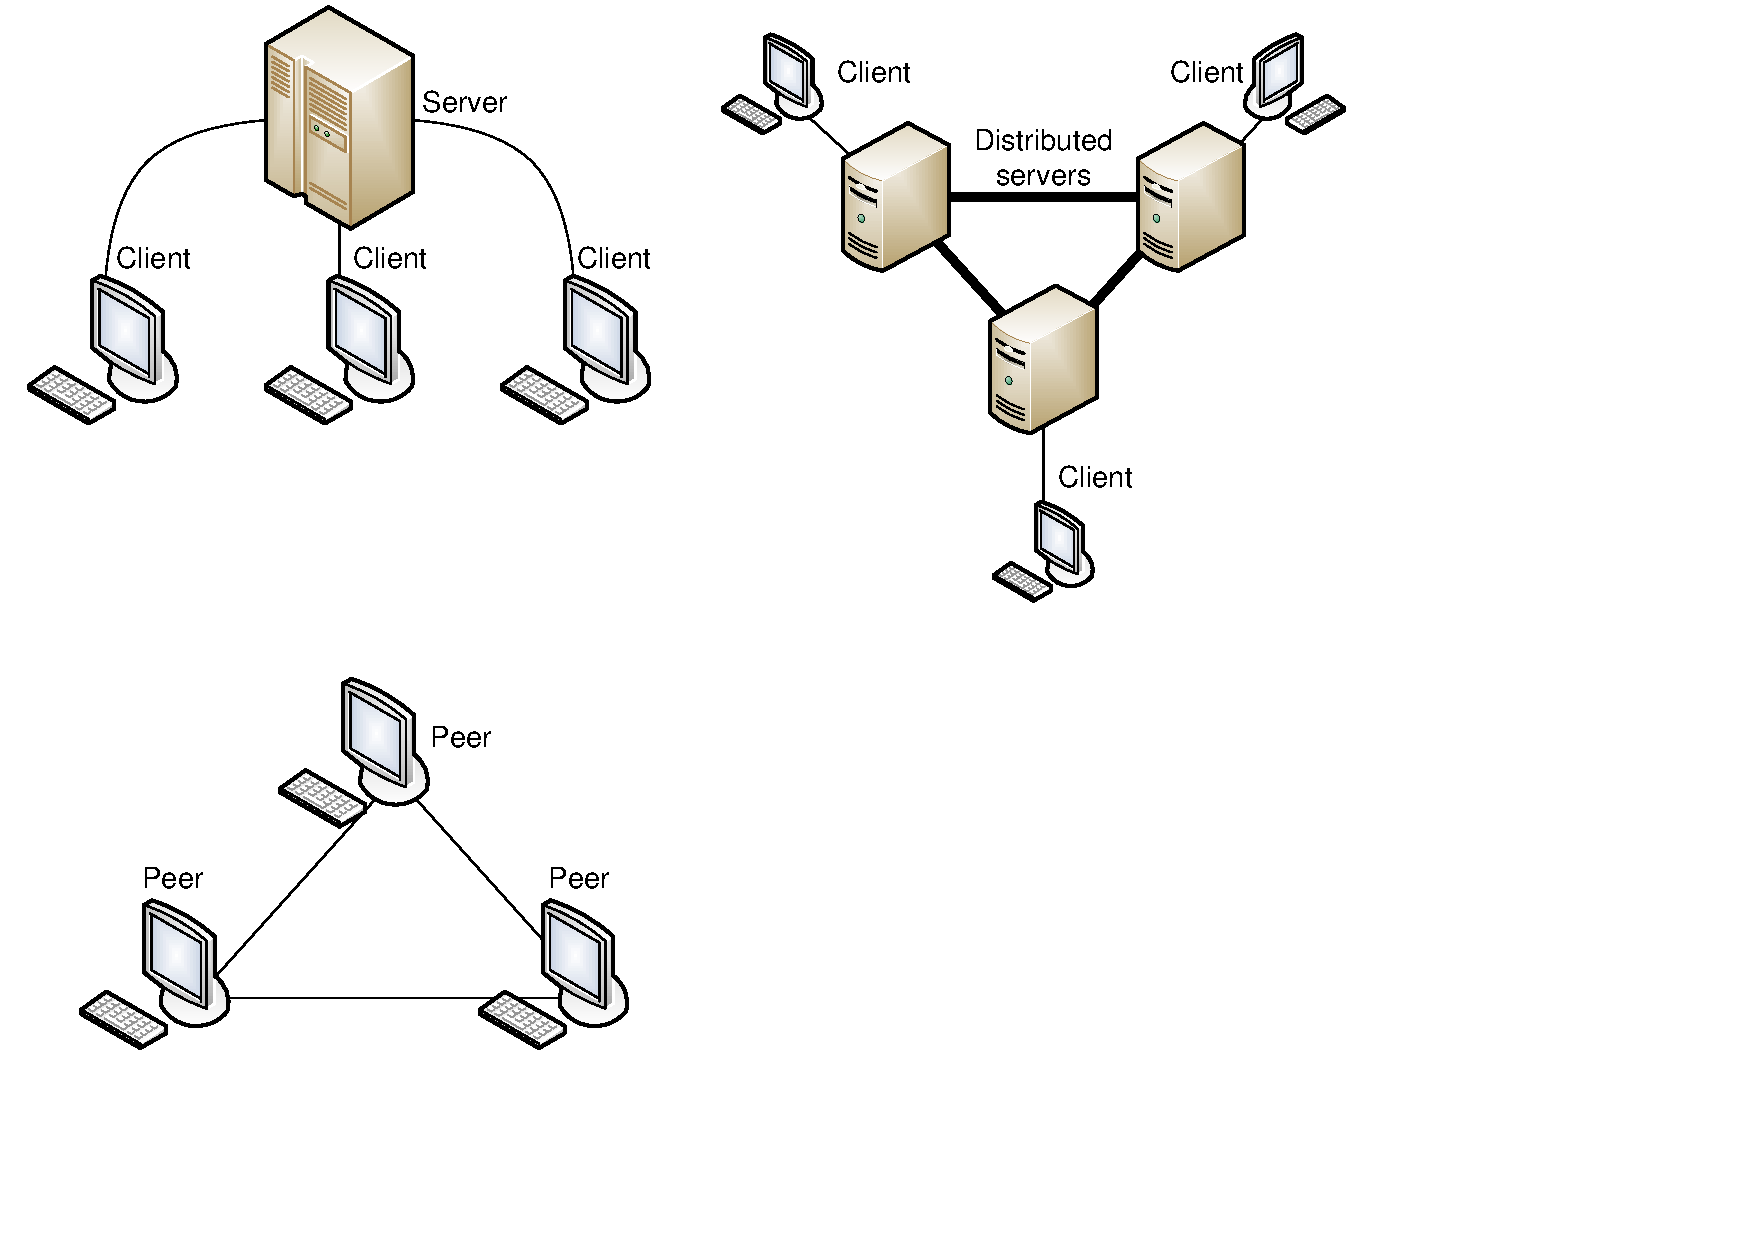
\includegraphics[clip=true, viewport= 0cm 12cm 11.5cm 21.5cm, width=0.5\columnwidth]{network_archs}}
\subfloat[Client/Multi-Server]{\label{fig_cms_arch}
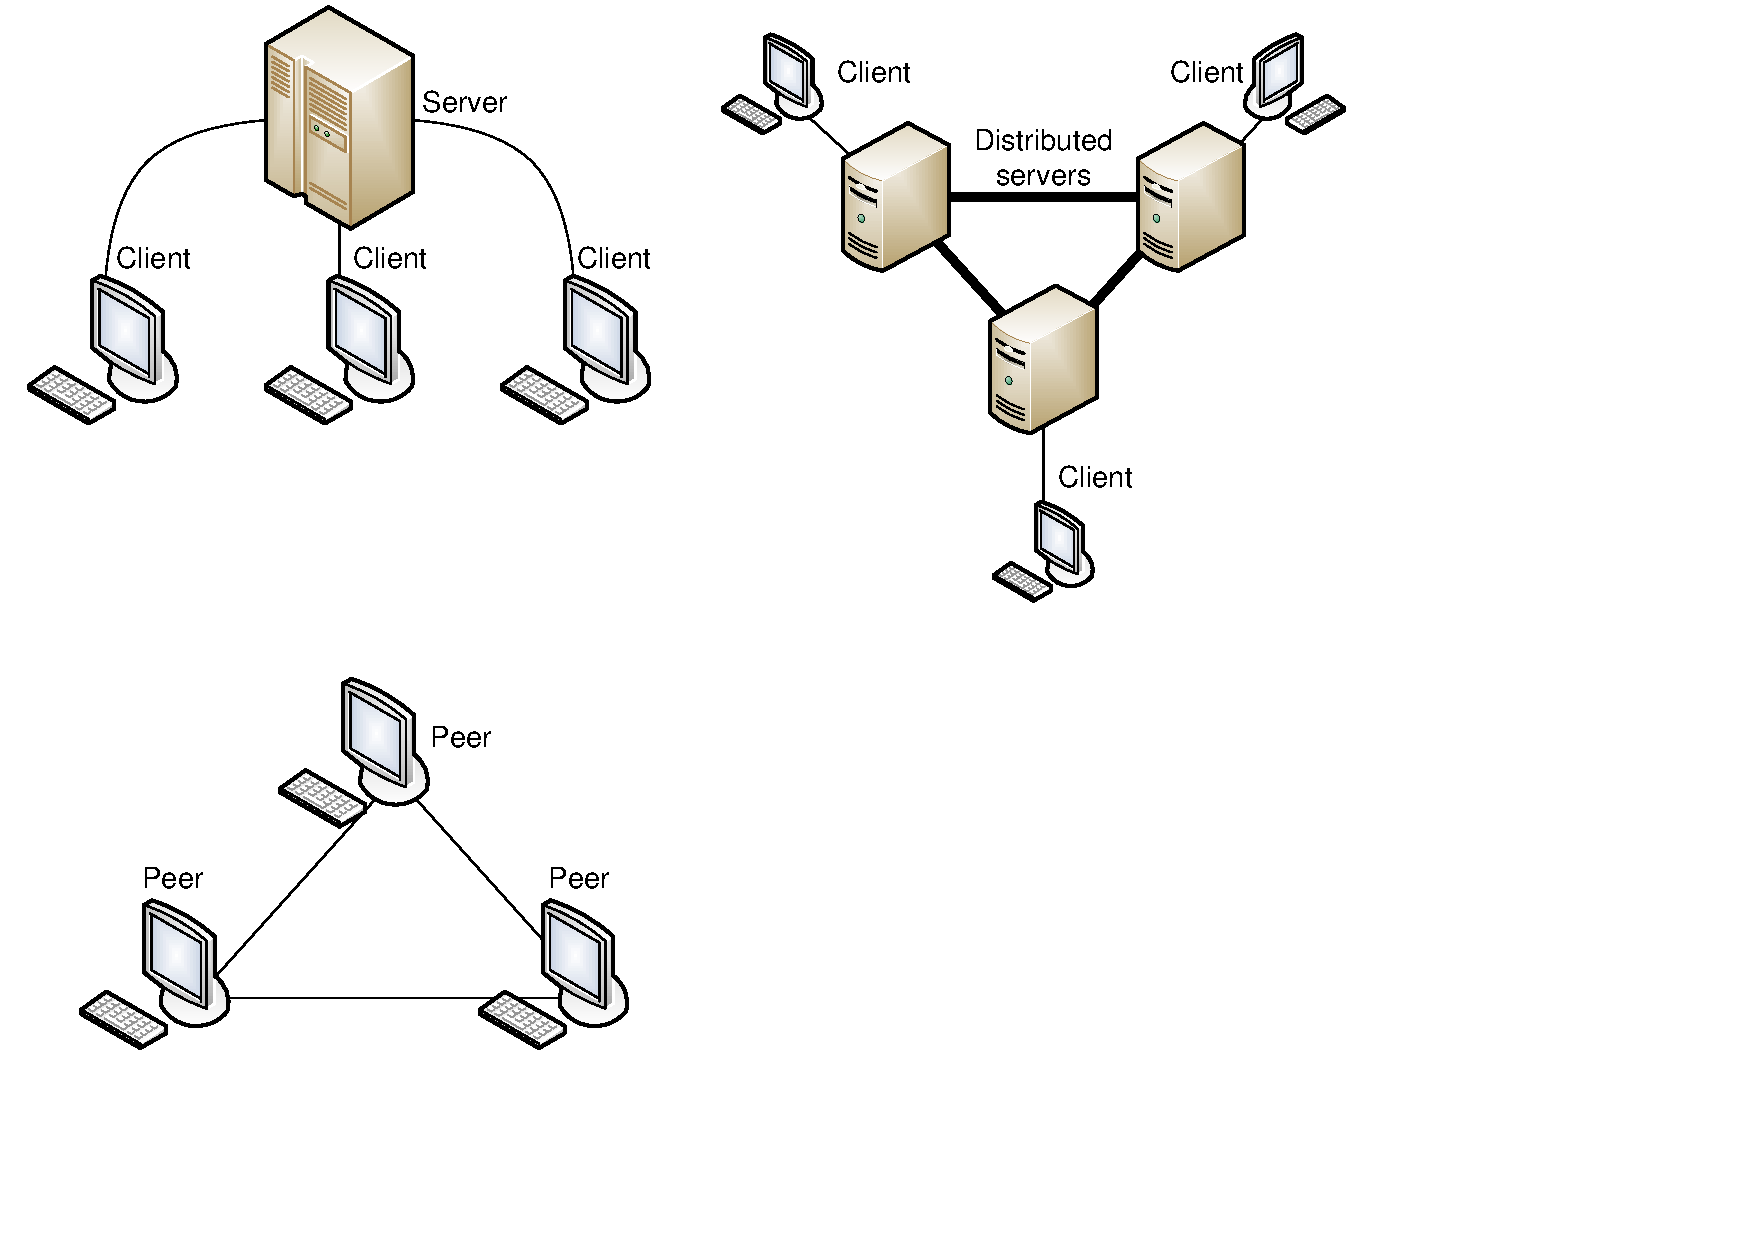
\includegraphics[clip=true, viewport= 12cm 10.5cm 23cm 21cm, width=0.5\columnwidth]{network_archs}}
\caption{Network architectures}
\end{figure}

Figure \ref{fig_cs_arch} shows the C/S model. The server is the entity on which the MMOG is hosted and is controlled by the game operator. Clients are computers operated by players, that connect to the server to play the game. The server is responsible for handling all queries from clients. Clients never communicate with other clients; they send their actions to the server and receive the updated states of other players from the server.

\subsubsection{Advantages}

The C/S architecture has two main advantages that has made it the architecture of choice for all MMOG developers. Because of the centralised approach of the architecture, both administration and security are greatly simplified. Administration is simplified, because the game operator has full control over the server, server data and code. Efficient logging is also supported, because the server is able to not only log all server actions, but also all client actions.

Security is a significant issue in MMOGs, since some players sell in-game currency for real-world currency \cite{chinese_gold_farmer}. This makes the MMOG a platform that is capable of producing income, which increases the incentive of players to gain an unfair advantage over others. The more popular an MMOG, the greater the security threat. Because the operator has full control over the server code and is never required to furnish the
client with the server code, a potential attacker never has any knowledge of the server architecture and code. Because clients are never allowed to communicate, all malicious users can be filtered out of the network by the server when detected and even banned from the network.

Operators are able to ban players, since these games usually require a game account, which is linked to a copy of the game as well as some payment method. This introduces a large cost to players whose accounts are banned. The server or cluster is also housed in a secured location, where access can be controlled. These factors simplify the security of the C/S model by allowing the developers to place all intelligence in the server.

\subsubsection{Disadvantageous}
\label{classic_cs_disadvantages}

The C/S architecture, however, does have some disadvantages. These are: weak robustness, weak scalability, high cost to the operator, high latency, high amount of required server bandwidth and weak handling of transient loads.
\begin{itemize}
\item The robustness of the system is weak because it is a single point of failure. If the server fails or goes down for maintenance, the game is off-line and players are unable to play.

\item The system is also weakly scalable, since a single server cannot easily be extended with more resources. Even if an off-line approach is used, where hardware is upgraded after the system is taken down for maintenance, the hardware required to support a game hosting more than 3000 players, become prohibitively expensive, as described in Section \ref{mmog_cost}.

The server hardware should be able to support peak system loads, which means that sufficient resources should always be provisioned to support these peak load. This is not an economically viable solution, because resources to handle peak loads are not used most of the time. This translates to operators paying for the provisioning of resources, without having active players that pay for these resources.

\item Because no clients are allowed to communicate with other clients, every change that is made to the game world by a client, first had to be communicated to the server, which in turns relays this message to all clients after applying game logic and artificial intelligence (AI) algorithms. This two hop path, with the additional time for computation added by the server as well as possible buffering at the server when many clients communicate, significantly increases the latency of the system compared to a system where direct communication is used.
\end{itemize}

\subsubsection{Client/Multi-Server}

In an effort to address some of the C/S issues, the distributed C/S, also called the Client/Multi-Server (C/MS) model, was introduced, shown in Figure \ref{fig_cms_arch}. In a C/MS model,
the server functions are distributed amongst multiple machines to distribute the server load.

In general, the issues addressed and improved by the C/MS architecture are robustness, scalability, and peak load handling. The system is more robust, because the failure of one server will not necessarily lead to the failure of the whole system for certain system designs. The system is more scalable, because many less powerful servers may be used, which allows for the hosting of more players than what is currently possible with single server hardware. It also handles transient loads better, because, for cases where loads can be predicted, resources can by moved between servers to improve the user experience.

The disadvantages of this system is that the administration complexity is greatly increased. Such systems, although capable of handling many more users than a single server, is also more expensive. These disadvantages are, however, not technical problems and so it is assumed for current games, that these systems are what is required if a game is to be hosted for a large number of players.

\subsection{The cost of doing business}
\label{mmog_cost}

With the fast growing MMOG market, many companies are spending a significant amount of money to produce premium MMOG titles. Some development cost estimates are: \$18 mil. for Aion, \$20 mil., for Everquest \cite{aion_everquest_cost}, \$63 mil. for World of Warcraft \cite{wow_cost} and \$100 mil. to \$200 mil. for Star Wars: The Old Republic \cite{star_wars_cost_1}, \cite{star_wars_cost_2}. Although these figures are purely estimates, it does show that to develop a premium MMOG title costs a lot of money.

The issue with MMOG development is that, although they cost more to develop than single player or smaller scale multiplayer games, they are just as likely to fail. Despite this, game publishers are spending a lot of money in an attempt to recreate the success that is World of Warcraft.

Because of the large revenues being generated from MMOGs, many competitors are entering the MMOG space. Currently, the rate at which new MMOGs are added to the market is outstripping the growth of the market itself \cite{newzoo_mmo_report}. Furthermore, because of the recession, over the past two or three years, game subscriptions have been shown to stabilise or even decline \cite{mmo_growth_chart}.

The significant initial investment required to develop an MMOG also doesn't present the complete picture. Another factor driving up costs for an MMOG is the money required for server hardware, maintenance and support. An MMOG is not finished when it goes live. A team of developers is required to maintain the game, release patches fixing bugs and to produce more content to keep the player base sufficiently interested to ensure that players will continue to pay \$15 per month to play. Development and maintenance costs for World of Warcraft for four years is estimated at \$100 mil. to \$200 mil. \cite{wow_cost}.

With the costs involved, it is therefore difficult for a new developer to enter into this space. After the large initial investment into the game's development, all server hardware must be acquired and staff appointed to maintain the game. This money is spent before it is known whether the game will succeed or fail. It has been estimated that during the lifetime of an MMOG, 80\% of the game revenue goes into hardware and maintenance costs \cite{cs_mmog_cost}.

\subsection{The peer-to-peer proposal}

In 2004, an architecture using the peer-to-peer networking model to host MMVEs was proposed by Knutsson et al. \cite{knutsson_p2p_first}. This
revealed a new research field, which attempts to establish the peer-to-peer (P2P) model as a viable alternative to the classic C/S and C/MS
architectures. P2P MMVE forms the focus of this work. There are various advantages to moving from C/S to P2P in MMVEs. These include: increased robustness, improved scalability, lower operator costs, improved handling of transient player load and lower latencies. The advantages are described in Section \ref{p2p_mmve_advantages} in detail,
but firstly it would be beneficial to acquire a greater understanding of the basics of the P2P network model.

\section{Peer-to-Peer systems}

A P2P network is a distributed network that exists out of many participating nodes to fulfil some objective. In this work, a P2P network is defined as being a distributed network with the following properties
\cite{Rodrigues_acm_comms_p2p}:
%
\begin{itemize}
\item \emph{High degree of decentralisation}:  No or little centralised control exists. Server functionality is distributed amongst all peers.
\item \emph{Self-organisation}: Little or no self-organisation is required in the network. Nodes are given an initial IP to allow them to join the network, but thereafter new neighbours are automatically acquired and nodes remain connected to the network, even with other nodes joining and leaving.
\item \emph{Multiple administrative domains} Peers are not under the control of any single authority. Peers in the network belong to different organisations or individuals and direct administration is impossible.
\end{itemize}

P2P systems have been popularised by mainly three systems developed in 1999: the Napster music sharing service, the Freenet data store and the SETI@home volunteer-based distributed computing project. These three projects highlighted the advantages of P2P networks being: low barrier to entry, scalability, resistance to faults and attacks, and an abundance and availability of resources.

\subsection{The OSI model and P2P overlays}

A basis of computer networking is the layered architecture model, called the open systems interconnection (OSI) model \cite{OSI_protocol_stack}. It defines various protocol layers that allow for abstraction of complex operation in the lower layers in the higher layers. The OSI layers are, from bottom to top: the physical layer, the data link layer, the network layer, the transport layer, the session layer, the presentation layer and the application layer. In practice, the session, presentation and applications layers are usually all folded into the application layer.

The physical layer is the physical transmission medium and carries physical signals. Physical level protocol standards include: IEEE 802.11 (Wi-fi), USB, Bluetooth, etc.. The data link layer, sometimes referred to as the MAC layer in the Internet protocol stack, carries frames and is responsible for point-to-point data transfer on the same local area network (LAN). Signals from the bottom layer are converted into bits and sequences of bits are grouped into frames, which is seen to be sent over the data link layer. As can be seen, every higher layer abstracts elements of the lower layer to reduce complexity.

The network layer allows communication between different LANs, using routers, gateways and host addressing. Every computer in a network is referred to as a host. A well known network layer protocol is the Internet protocol (IP), which routes all Internet traffic. The transport layer is referred to as the end-to-end layer and represents the abstract connection between a source and destination host, where all intermediate routers and LANs may be ignored, since they are abstracted away by the network layer. Well known protocols in this layer include the user datagram protocol (UDP) and transport control (TCP) protocol. Above the transport layer, for the purposes of this work, is the application layer. The application layer has access to all network services, including routing and reliable transmission.

In the C/S architecture, the client and server are both located in the application layer and communicate with each other using the transport layer. They need not be aware of any of the lower layers.

P2P networks are created and maintained in the application layer of the OSI model, called the P2P overlay. An overlay is required so peers may know which other peers are part of the P2P network, since most nodes on the Internet will not be part of the network. The overlay is then defined by the routing table information stored on each peer. The overlay can be thought of as an additional layer in the OSI model. The overlay interfaces with the transport layer and P2P applications are one layer higher and communicate by using the overlay.

Peers in an overlay network might have neighbours that have no relationship to their physical position in the underlying network.

\subsection{Structured and unstructured P2P overlays}
\label{overlays}

Overlays can broadly be classified into structured and unstructured types. The classification is mostly based on the differing methods of routing and content retrieval in the network. This section only provides a brief comparison between structured and unstructured overlays. For a detailed comparison between the two types that also deals with many of the myths of structured overlays, please refer to \cite{Castro_structured_overlay_myths}.

With unstructured approaches, one is never assured that a data item will be retrieved, even if that data item is present in the network. If many duplicates of a data item are contained in the network, this becomes less of a problem, since it is assumed that the request will be routed to some set of nodes that do  possess the item.

An unstructured architecture is well suited to content sharing and Voice over Internet Protocol (VoIP) networks, for example: P2P TV, BitTorrent, Gnutella and Skype. The reason for this is the high level of duplication in these networks, especially for popular content. It is also easier to perform keyword searches in unstructured networks and the overlay requires less maintenance.

Structured overlays have been proposed that provide for efficient routing and reliable retrieval of data items. Some of these well known overlays are: CAN \cite{CAN}, Chord \cite{chord}, Tapestry \cite{tapestry} and Pastry \cite{pastry}. The basic principle of a structured overlay is that all nodes are identified by unique identifiers (IDs).

A popular method to create the IDs is to use hashes to a circular key space, using for example, the SHA-1 hash function. Any node in the overlay network is then able to efficiently route a query with a given ID, to a node with an ID closest to the given ID. An accurate comparison is that unstructured overlays are good at finding ``hay'', while structured overlays are good at finding ``needles'' \cite{Rodrigues_acm_comms_p2p}.

\subsection{Features of structured P2P overlays}

A structured P2P overlay has certain key features that determines its lookup speed, space consumption and bandwidth requirement \cite{p2p_networking_handbook}. These features are geometries, routing algorithms, join/leave mechanisms, routing table maintenance and bootstrapping.

\subsubsection{Geometries}

An overlay's geometry determines how nodes are structured in the application layer network. The geometry allows for deterministic routing. The geometry determines the number of required lookup hops and how the network will be maintained during times when nodes join and leave the network, called churn.

\subsubsection{Routing algorithms}

The routing algorithm is directly related to the specific overlay geometry. The routing algorithm determines which nodes are traversed when a message is sent to a target node. The routing algorithm and the geometry determines the number of expected hops for a message to reach a destination.

\subsubsection{Join mechanism}

P2P networks experience constant churn, where nodes are joining and leaving the network. Mechanisms for a node to join the network should be present. This is usually in the form of a well known directory (boostrap) server. When a node wishes to join the network, the directory server sends a set of nodes that the node may want to join.

\subsubsection{Leave mechanism}

If a node leaves the overlay, its neighbours have to be informed so they may update their routing tables. This is termed \emph{routing table maintenance} and has to happen every time a peer leaves the network. Neighbouring nodes of a node that left the network might also have to inform their neighbours of the change. Two types of routing table maintenance exist: opportunistic and active maintenance.

Opportunistic maintenance attaches routing information to existing request packets. Routing data is essentially ``piggy backed'' onto existing messages. This reduced messages overhead but the rate of routing table maintenance is directly proportional to the message rate. Active maintenance makes use of explicit update messages, which required more bandwidth but is more reliable.


\subsubsection{Bootstrapping}

After having been informed of a peer to join, a joining peer may initiate the process of positioning itself in the P2P network, called bootstrapping. This is the process of finding out where the joining node fits into the overlay in terms of the geometry. If the overlay requires that all nodes be connected in a ring organised by ID, then the joining peer must discover the nodes whose IDs are one more and one less than its own and join those two peers.

The process of bootstrapping is complete when a joining peer becomes a functioning member of the P2P overlay.

%TODO: Add something about the effect of the hashing and why it's important

\subsection{Advantages}

\begin{itemize}
\item P2P networks have a low barrier to entry, since little or no centralised infrastructure is required to maintain the system. This makes P2P networks inexpensive to operate and is one of the reasons Napster was able to provide its service for free.

\item P2P networks are considered scalable. Pure P2P networks can theoretically grow from hundreds to millions of nodes, with the service remaining functional. This is all possible without the need for the operator to acquire more infrastructure, as opposed to the centralised client/server network, which required more powerful server clusters are the network grows to handle the growing number of client requests.

\item A P2P network is also resistant to faults and attacks, since the failure of a single node has little to no effect on the network. This is because there are usually few nodes that are critical to the correct functionality of the system. To incapacitate a P2P network, an attacker usually has to shut down a large proportion of the network.

\item Not only does a P2P operator not require its own infrastructure, but the P2P infrastructure that forms part of the network and consists of peer machines provide abundant and highly available resources, being computation power, long term and short term storage. This means that P2P networks can be designed to run on powerful computers.
\end{itemize}


\section{Peer-to-Peer MMVE network architectures}
\label{p2p_network_architectures}

P2P MMOGs are considered a sub-class of P2P Massively Multi-user Virtual Environments (MMVEs), a class that also includes large scale military simulators.

This architecture does, however, still have a few major issues that need to be solved before MMVEs can be developed that use it. If
these issues, discussed in Section \ref{key_challenges}, can be solved, a P2P architecture holds some powerful advantages over a C/S system.

The core idea of the P2P model is that each peer contributes sufficient resources to the network to host itself. This also means that all functions of the server in the classic C/S model are distributed amongst all peers.

\subsection{Advantages}
\label{p2p_mmve_advantages}

\begin{itemize}
\item The P2P architecture is robust, because there is no server that can fail, only individual peers. Individual peers failing will not affect any other peers other than the peer that failed. This behaviour makes game down-time extremely unlikely.

\item The system is scalable, because every peer hosts itself.

\item Because of the high scalability, no extra resources are required from an operator perspective, when more peers join the network.

\item P2P networks also efficiently handle transient loads, since the joining peers contribute their own resources. If many players suddenly enter the
game no resource provisioning issues will arise, since peers already possess the required resources.

\item P2P architectures create a lot of opportunities for independent developers, because a large initial investment is no longer required to purchase
the expensive server hardware. Not only are hardware costs reduced, but running costs are also reduced.

\item Bandwidth required by the game server is now shared amongst users, which means that very little bandwidth costs will be incurred by the provider.

\item Latency is improved, because it is now possible to directly communicate between peers and it is not necessary to communicate via a server.
The distribution of the load as well as direct communication will further reduce latency.
\end{itemize}

\subsection{Requirements}

Key requirements have been identified for the creation of a P2P MMVE. What follows is an expansion and reinterpretation of the requirements identified by Schiele et al. \cite{Schiele_p2p_requirements}.

\subsubsection{Distributed computation}
\ref{distributed_computation_requirement}

Non-Player Characters (NPCs) are characters that are not controlled by any human player, but are rather controlled by some artificial intelligence routine or script executing on some host machine. These characters represent the traders and monsters in MMVEs and usually contain sets of rules that determine how they should interact with Player Characters (PCs) as well as their own state information. An NPC's state can be how much money and items it has to trade or how much health it still has after being attacked by a player.

Some game objects require computational power to function. An example of this is the Artificial Intelligence routines of NPCs or the computation of physics effects on in-game objects. In P2P MMVE, it might be required to distribute these computational tasks to offload computation load from peers that do not have sufficient resources.

\subsubsection{Consistency}
A key challenge with any networked game is how to maintain state consistency between users in the virtual world. In other words, to ensure that all users perceive a virtual world in the same state. Solving the state consistency problem for P2P MMVEs is one of the major development challenges and forms the focus of this work. The challenge of state consistency will be described in detail in Chapter \ref{chp:CONSISTENCY}.

\subsubsection{Persistency and state management}

\subsubsection{Self-organisation}\
Handling of user churn

\subsubsection{Availability}
Game must always be online (P2P requirement)

\subsubsection{Interactivity}
Low latency interaction and masking latency with dead reckoning

\subsubsection{Scalability}
Server and peer bandwidth requirements

\subsubsection{Security}

Security, which includes cheating mitigation, has been identified as a major issue for P2P networks \cite{knutsson_p2p_first}, \cite{challenges_p2p_gaming}, \cite{cheat_proof_event_ordering}. The challenges reside in the fact that peers are not under the control of the game producer. Since all server data are distributed amongst peers, all peers have access to sections of the server data. Peers also have access to the distributed server code. One advantage that can be exploited to prevent cheating is that no peer contains all server data and no single peer has more authority than another.

\subsubsection{Efficiency}
The peer must efficiently implement the server, since it still has to be a client as well

\subsubsection{Maintainability}

\subsubsection{Incentives}

P2P schemes require all players to share resources in order to ensure correct functionality. Players might, however, not want to share their resources, whilst still benefiting from the resources of others. The purpose of incentive mechanisms is to ensure that all players contribute resources, by incentivised contribution.

All distributed resource sharing models require incentive mechanisms. For example, Bittorrent systems use the tit-for-tat protocol to ensure that all people downloading data are also contributing data \cite{tit_for_tat}. Such mechanisms are also required with P2P MMVEs. One advantage in designing an incentive mechanism for a P2P MMVE is that players can be made to contribute resources for the duration of play. The issues with file sharing systems are not present where a peer, after downloading a file, has no more incentive to contribute.

\subsubsection{Structured P2P overlay}

Because there is no assurance that a data item might be retrieved from an unstructured network, especially when that item is scarce, unstructured overlays are not considered adequate as a basis for P2P MMVEs, where all data items must be available at all times.

A P2P MMVE architecture requires a structured P2P overlay in the broad sense. In P2P MMVEs, peers have to be connected in some geometry and it should be possible to route messages between peers. P2P MMVEs require a bootstrapping server to enable peers to join the network and be placed in it. A P2P MMVE architecture should handle churn with a minor impact on system operation. Most importantly, all objects stored in the P2P MMVE should be available at all times.

\subsection{Key challenges}
\label{key_challenges}

Using P2P MMVEs has many advantages, some challenges still remain. The main challenges are state consistency, limited peer bandwidth, cheating mitigation, incentive mechanisms and distributed computation. This section will present some information on work that has been done in the different areas and talk about the maturity of the various solutions. In general though, most solutions are still research projects and none have yet been implemented as commercial products.

\subsubsection{Peer bandwidth}

In a paper by Miller and Crowcroft, a packet simulator was created to determine the required bandwidth and effective latency, if a game such as World of Warcraft were to be implemented using P2P technologies \cite{Miller_p2p_infeasability}. Their simulation results indicate that today's networks are not able to host P2P MMVEs, with the required bandwidth and latency constraints. Such a significant result requires verification, but at the least, it shows that reducing bandwidth and latencies for P2P MMVEs should be a primary design requirement.

\subsubsection{Cheating mitigation}
\label{key_challenges_cheating}

%Describe "server data" in terms of a more generic form to be able to have that generic form in the server and p2p architecture.

There are various security issues that are usually classified according to the level in the OSI protocol stack where they occur. The areas identified by \cite{cheat_proof_event_ordering} and expanded upon by \cite{cheating_taxonomy} are: game level, application level, protocol level and infrastructure level. The description is consistent with the generally used layered security model \cite{distributed_systems_security}.

\begin{itemize}
\item Game level cheats are ways in which a malicious player may gain an unfair advantage over other players, within the confines of the game. These cheats are usually because of software bugs and some examples are duplication and teleport cheats.

\item Application level cheats are where malicious players alter the game software to gain an unfair advantage. This is usually done by gaining access to the game state to which they should not have access at the current time. An example of this is ``map reveal'' cheats in strategy games, where the ``fog of war'' is removed and the player can observe all the opponent's movements. Other cheats that are used include augmenting the player's UI with extra information that allows the player to make more informed decisions.

\item Protocol level cheats are cheats based on the different methods of communicating data across the system. These usually concern dropping, delaying of modifying IP packets to achieve certain outcomes in the game.

\item Infrastructure level cheats concern exploiting the underlying infrastructure on which a game is built. Types of infrastructure cheats include denial of service (DOS) attacks on the P2P overlay to prevent messages that should be forwarded by a peer from being forwarded.
\end{itemize}

As with all taxonomies, all cheats may not cleanly fit into one if these boxes, some cheats may occur over multiple levels or a cheat with a specific outcome can be implemented differently on different levels. The field of P2P security has recently received more attention than in the past and has started to bear fruit \cite{survey_p2p_game_cheats}.

This is, however, an ongoing research field with many issues still open. For an in-depth review of the security issues facing peer-to-peer system in general, refer to \cite{p2p_security_issues}. These issues are the same issues facing P2P MMVEs, with the exception of the game and application layer issues.

\subsubsection{Incentive mechanisms}

Some proposed incentive schemes increase a player's reputation when resources are provided  \cite{classic_p2p_reputation} \cite{proactive_reputation}. This might create a type of meta game, where players try to gain as much reputation as possible. It can however be argued that this scheme does not really enforce the provisioning of resources. A player who does not want to provide resources might not see a higher reputation as sufficient incentive to provide resources.

Other issues with incentive schemes is that sometimes players might have insufficient resources. Such players should be aided by other players with sufficient resources and not be disallowed from playing the game. When limited resources are taken into account, the issue of reporting a false amount of available resources becomes a problem. A peer that has sufficient resources, might report insufficient resources, to avoid being penalised. It is evident that there is a need for more research in this field.

\subsubsection{Distributed computation}

Some architectures assume that the computational requirements will be fulfilled where the object state is hosted \cite{solipsis}, but other schemes exist that allow for the CPU power to be distributed amongst peers. One such scheme makes use of a ``job board'' like mechanism, where tasks are advertised on specialised peers. All peers monitor these specialised peers and may elect to perform the advertised tasks \cite{fan_mediator_paper}.

\subsubsection{State consistency}

The state of the art of state consistency techniques will be reviewed in detail in Chapters \ref{chp:CONSISTENCY} and \ref{p2p_MMVE_state_persistency}.

\section{Research objectives}

\section{Related work}

\section{Contributions}
\label{objectives}

\begin{itemize}
\item A generic state consistency model is developed that encompasses both C/S and P2P consistency models.

\item A review of various state management and state persistency systems is performed.
    \begin{itemize}
    \item The state management survey identifies some key metrics by which state management systems may be compared.
    \end{itemize}

\item A novel state management and persistency architecture, called Pithos, is proposed and implemented in simulation, which increases reliability and responsiveness compared to classic state persistency methods.
    \begin{itemize}
    \item Multiple methods of implementation are described that provide different benefits, depending on the situation.
    \item The various implementation methods are evaluated and recommendations are made on which methods work better in which situations.
    \end{itemize}

\item A statistical model for expected object lifetimes is developed and used to verify the Pithos results.
\end{itemize}

\begin{itemize}
\item Early in the literature study phase, it was discovered that no research projects that deal with P2P MMVEs present the complete picture of the field. A significant amount of research has been done in the field of state consistency (reviewed in Chapter \ref{chp:CONSISTENCY}), but in this field, no model has been provided which shows what is required to build a complete state consistency architecture. The first contribution of this work is to provide such an architecture at the start of Chapter \ref{chp:CONSISTENCY}.

\item The generic consistency model that is developed is not only applicable to P2P MMVEs, but to any networked virtual environment that required state consistency. The generic consistency model is also compared with well known client/server and P2P consistency models, to show how the existing models can be seen as more specialised versions of the generic consistency model.

\item After developing a generic consistency model, this work then focusses on an area of state consistency that has received little attention from the research community, namely: state management and state persistency. This area is concerned with managing object states as they are updated by events occurring in the virtual environment. Also during a literature review of this field, it was found that no thorough review of this field has been done to compare the different types of storage systems present in P2P MMVEs and presented in the literature. We then preceded to perform such a review, presented in Chapter \ref{p2p_MMVE_state_persistency}. The results of this survey has also been published in the IEEE Transactions of Parallel and Distributed Systems \cite{gilmore_p2p_mmog_state_persistency}.

\item During the survey, some key metrics were identified by which state management and state persistency systems may be described. A proposal was also made as to how these metrics may be measured. What was found upon completion of the survey is that no storage system has thus far been created to satisfy all identified metrics. Work was then undertaken to develop a novel state management and persistency architecture that satisfies all identified requirements.

\item The state management and persistency architecture has been developed and called ``Pithos''. Pithos has been implemented in a network simulation framework, called Oversim, which runs on the Omnet++ simulation environment. The Oversim framework itself has also been extended to implement our novel generic consistency architecture. Pithos has been implemented in the root object store section of this architecture.

\item Many of the key mechanisms in Pithos, such as object retrieval, have been implemented using multiple methods. These methods are then compared to determine the advantages and disadvantages of each. Pithos is also compared to the storage systems identified. Pithos always shows similar or improved performance over classic storage systems in all identified areas.

\item In order to verify the correct functioning of Pithos, mathematical models are also developed to describe Pithos's performance in the various identified metrics. Amongst these is a novel Mathematical model that makes use of an embedded continuous time Markov chain to determine expected object lifetime for varying amounts of network churn, various network sizes and replication rate. The mathematical model is compared with actual Pithos results and appears to match almost exactly.
\end{itemize}

\section{Summary of this work}

Chapter \ref{chp:CONSISTENCY} presents an overview of state consistency models. Initially, it describes the general process by which state consistency is achieved. Some classic consistency models are then presented in terms of the generic model. Consistency models for P2P MMVEs are then presented, with an overview of work that has been done in each of the various sections required to implement a complete consistency model.

Chapter \ref{p2p_MMVE_state_persistency} focuses on the state management and state persistency aspect of P2P MMVE state consistency. Initially, some metrics are defined according to which different storage architecture may be compared. A literature review is then presented, where papers that deal with various storage techniques are grouped and the advantages and disadvantages of each group is then discussed. This chapter also identifies a need for a novel state management and persistency architecture.

Chapter \ref{chp:DESIGN} describes the design and implementation of Pithos, the novel state management and persistency architecture. Initially, the overarching Pithos design is described, including the perceived use case and design goals. The Oversim simulation environment is then described, along with the extensions that were made to model the generic consistency model. The Pithos implementation is then described in terms of Oversim modules. Key mechanisms that implement that Pithos design are then presented with reference to the Pithos Oversim modules. Various methods to implement some mechanisms are descried.

Chapter \ref{chp:EVALUATION} evaluates the Pithos implementation. The performance of the key mechanisms are presented and the various implementation methods are compared. Pithos is also compared with other storage implementations.

Chapter \ref{chp:MODELLING} models Pithos's performance with reference to the identified metrics for P2P MMVE storage systems. A focus is placed on expected object lifetime and a novel model is developed, based on an embedded continuous time Markov chain.

Chapter \ref{chp:VERIFICATION} compares model results with Pithos simulation results. The purpose of this chapter is to verify the correct functionality of Pithos, according to mathematical models. The chapter also explores how to design storage systems with desired object lifetimes.

Chapter \ref{chp:CONC} concludes the work. It presents a summary of the work, lists contributions made and discusses some future areas of research.

\include{contents/Lit_study}
\include{contents/System_overview}
\include{contents/Link_acq}
\include{contents/system_design}
\include{contents/detail_imp_test}
\chapter{Conclusions and Recommendations}
\label{chp:CONC}

This work focussed on developing a state management architecture for P2P MMVEs. In order to do this, an understanding was required of P2P networks, MMVEs and what the main challenges of P2P MMVEs are.  It was found that state management and persistency is used by the consistency architecture and, therefore, that the consistency architecture implicitly specifies the storage requirements.

After having identified the requirements of a state management and persistency architecture, related work was reviewed and compared against the identified requirements. This allowed us to identify areas where improvements might be made.

The design of Pithos was presented in order to satisfy all identified requirements, presenting every aspect of Pithos in terms of the requirement identified. The Pithos use case was reviewed and presented as a distributed storage system and the mechanisms to implement the use cases were discussed.

With the conceptual design finalised, the implementation specifics were reviewed. Pithos has been implemented as an Oversim simulation that allows for large scale simulations. Some implementation issues that were reviewed were maintaining group consistency as well as persistency in group storage. An evaluation was performed in order to verify that Pithos satisfies all the requirements originally identified.

When Pithos was evaluated for various churn levels and repair rates, it was seen that many factors influence reliability. The factors influencing reliability were found to be directly related to expected object lifetime. A Markov chain model was developed to allow for the prediction of expected object lifetimes. It was found that the literature reviewed assumed an infinite network size and does not take limited network sizes into account. Comparing our model with simulation results, it was found that finite group sizes does affect object lifetimes when the average group size is small, compared to the required number of replicas.

\section{State consistency}

The generic consistency model developed provides a framework for the design and development of MMVEs in general. Because many aspects of the generic consistency model are trivial in C/S models, the model is perhaps more applicable to a P2P MMVE

\section{State management}

\section{Pithos}


\section{Further work}
\label{further_work}


%==== Appendices ====================================================
\appendix
\appendixpage\relax

\chapter{Ensuring group consistency in Pithos}
\label{chp:GROUP_INCONSISTENCY}

This appendix described, in chronological order, the steps taken to ensure group consistency. It provides initial findings, discusses the reasons for inconsistency and introduces the proposed solutions.

\section{Initial approach}
The initial approach to achieve group consistency was to have every peer inform all other peers when it was moving from one group to another. If a peer is removed from the network due to churn, another peer has to discover that the peer has left, which is done with timeouts. If a request times out, the peer making the request informs the group of the peer that left.

\begin{figure}[htbp]
 \centering
 \includegraphics[clip=true, viewport=0mm 0mm 460mm 212mm, width=\columnwidth]{gc_first}
 \caption{Group consistency before any improvements}
 \label{fig_gc_first}
\end{figure}
%
Figure \ref{fig_gc_first} shows an enlarged view of the perceived group size of every node in the group for the initial group consistency scheme. The lines running across the graph is due to nodes leaving the network and joining again at a later time.

From approximately 2925 s, a new peer joins the group and reports the group size as eight, when all other peers report the group size as seven. Multiple variations of these inconsistencies occurred during testing. A primary source of inconsistencies was the fact that it takes time to inform all group peers of a peer that left and that it takes time to inform all group peers of a peer that joined.

Issues also occurred because of how newly stored objects are handled. When a new peer joins the group, it starts to generate objects. The group super peer sends a joining peer a list of group peers. After this occurs, the group peers are informed of the new peer. A peer joining a group can immediately start to store objects at the request of other peers. This can happen before some peers are aware of the joining peer. The unaware peers will then get a message saying that an object has been stored on the new peer, before they are aware of the new peer. The solution was to assume that an object was generated by a valid peer and to add any unknown peer information contained in an object add message to the peers list in the group ledger.

Group inconsistency can arise because there might be some latent object add messages still enroute to peers, after the peer has already left the network and informed other peers of its leaving. This means that a peer has already left, but after it informed the group peers of its leaving and all group peers have removed the peer from memory, the group peers receive a message for an object that is supposedly now stored on the peer that just left. The mechanism mentioned above is initiated and the, now unknown, peer is again added to the peer list.

Many transient group states that led to inconsistencies were solved by the super peer storing the information of the last peer that left and the last peer that joined. Every time a new peer joins, the super peer informs the joining peer of the last peer that left. This allows the joining peer to ignore any latent object add messages received from the leaving peer. Any messages received from the last peer that left are ignored. This prevents latent messages from peers that left to affect the group view of peers.

\section{Peer starvation problem}
\begin{figure}[htbp]
 \centering
 \includegraphics[clip=true, viewport=0mm 0mm 455mm 212mm, width=\columnwidth]{gc_middle}
 \caption{Group consistency with starvation}
 \label{fig_gc_middle}
\end{figure}
%
The mentioned improvements created the issue shown in Figure \ref{fig_gc_middle}, where a peer will believe that another peer has left. The group will be informed of the peer that supposedly left, but is actually still present in the group. Because all peers will now ignore messages from the peer that supposedly left, including the super peer, all requests sent by the peer that supposedly left will be ignored. The requests will then timeout on the ignored peer and the ignored peer will remove all group peers. This isolates the peer and prevents any requests from being serviced.

The starvation was caused by peers not responding to requests. A scenario could occur where a peer did not contain a requested object or where the network bandwidth was limited, which prevented a response from arriving at a peer before the request timeout expired. In either of these two situation, the peer making the request was under the impression that the target peer had left the network. It then informed all other peers of this.

The solution to this issue was to adjust the timeout as a function of the available network bandwidth and to make sure every node always responded to a request, whether as a success or failure. Functionality was also added to the super peer to check whether a peer that was reported as having left, actually did leave the network.

Other issues were caused when group migration was enabled. A node might leave a group to move to another, but as the node leaves some peer that has not been informed of the peer leaving would make a request form the leaving peer. The leaving peer would respond to that request, which would have the requesting peer add the peer back into the group. This could cause the situation where peers existed in multiple groups.

The solution to this was to include the group membership information in every request message. A peer's membership can be uniquely identified by the IP address and port of the group's super peer. If a peer receives a message with a different group address than its own, it ensures that that peer is not part of its group.

This also solved the case where Peer A requested an object from Peer B, just as Peer B was leaving the group. Peer B will already be in its new group when receiving the request from Peer A. Peer B will see that the request originated from outside its group, so will not add the new peer to its group. If it contains the requested object, it will however still respond with the object. When Peer A receives the object, it will detect that it was sent from another group and remove Peer B from its group ledger. In this way, the request was successfully handled and group consistency is maintained.

\section{Final solution}
\begin{figure}[htbp]
 \centering
 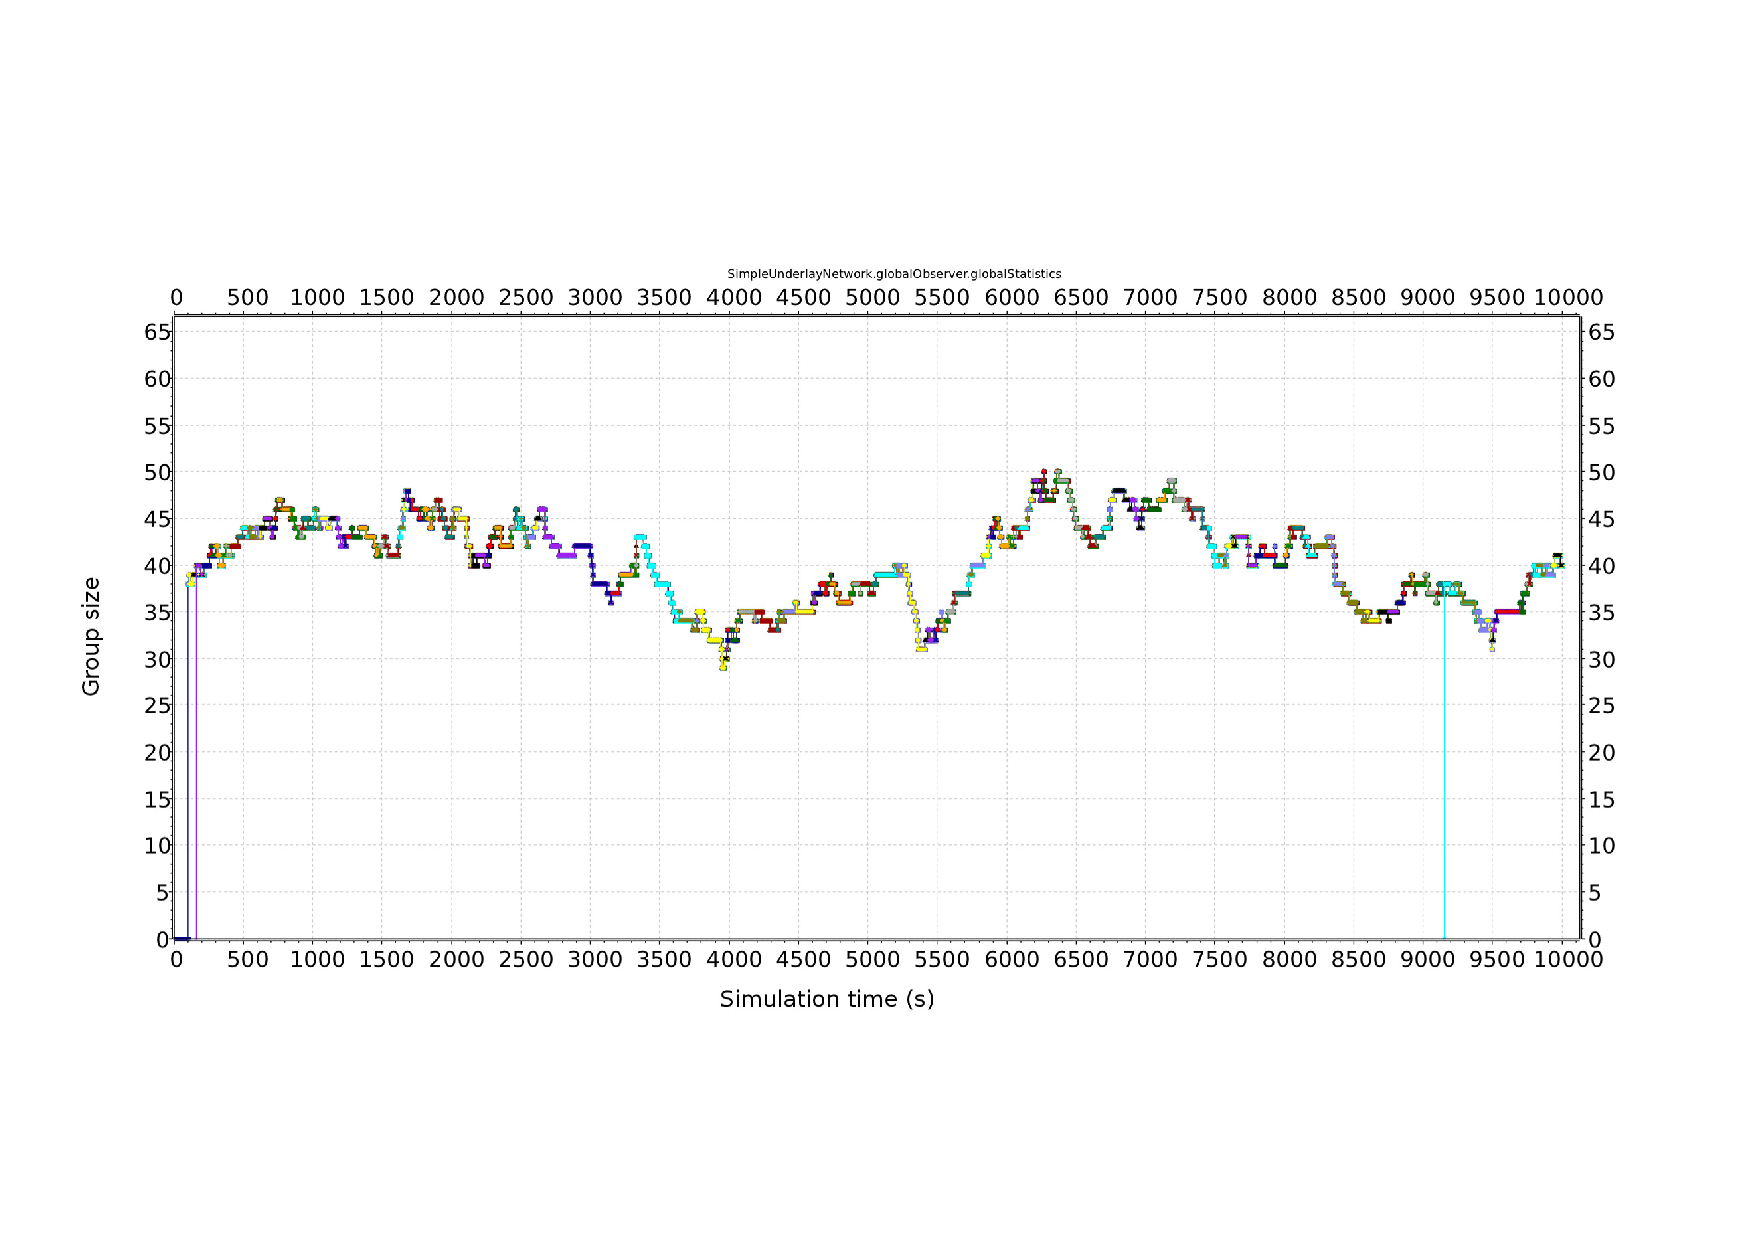
\includegraphics[clip=true, viewport=12mm 35mm 275mm 165mm, width=\columnwidth]{gc_final_png}
 \caption{Group consistency after all improvements}
 \label{fig_gc_final_app}
\end{figure}
%
Figure \ref{fig_gc_final_app} shows the group consistency after all improvements were added for a larger group than the previous two. Even with the larger group, complete consistency is achieved.

When object lifetime was tested, all requests were stopped after a certain period of time to speed up the simulation. This created an issue where group peers did not become aware of peers leaving the group, because no peers sent requests that could timeout. This prompted the addition of keep-alive messages.

Regular keep alive messages are sent to peers. If a peer does not respond to the message, that peer is removed from the group. The time between keep alive messages can be adjusted as a function of network churn. In order to reduce the load on the super peer, each peer randomly chooses a target peer and sends a keep-alive message, as explained in Section \ref{leave_design}.

%\chapter{Overlay storage configuration parameters}
\label{chp:OVERLAY_CONFIG}

\begin{table}[phtb]
\centering
\begin{tabular}{|r|l|l|l|}
\hline
Parameter                       & Low  & Medium & High  \\
\hline
Stabilise retries               & 1    & 2      &  3    \\
Stabilise delay                 & 10s  & 5s     &  3s   \\
Fix finger table interval       & 120s & 10s    &  5s   \\
Check predecessor delay         & 5s   & 5 s    &  3s   \\
Extended finger table           & no   & yes    &  yes  \\
Extended finger table candidate & N/A  & 3      &  4    \\
\hline
Join retries                    & 2    & 2      & 2     \\
Join delay                      & 10s  & 10s    & 10s   \\
Routing type                    & iterative & iterative & iterative \\
Successor list size             & 8    & 8      & 8     \\
Use aggressive join             & yes  & yes    & yes   \\
Proximity routing               & no   & no     & no    \\
\hline
\end{tabular}
\caption{Chord configuration parameters for the various test cases.}
\label{tab_chord_configs}
\end{table}

\begin{table}[phtb]
\centering
\begin{tabular}{|l|l|}
\hline
Parameter                       & Value\\
\hline
Bits Per Digit                  & 4\\
Number of Leaves                & 16\\
Number of Neighbors             & 0\\
Join Timeout                    & 20s\\
Ready Wait                      & 5s\\
Second Stage Wait               & 2s\\
Repair Timeout                  & 60s\\
Enable New Leafs                & no\\
Optimize Lookup                 & no\\
Partial Join Path               & no\\
Use Regular Next Hop            & yes\\
Always Send Update              & no\\
Use Discovery                   & no\\
Ping Before Second Stage        & yes\\
Discovery Timeout Amount        & 1s\\
Routing Table Maintenance Interval & 0s\\
Send State at Leafset Repair    & yes\\
Override Old Pastry             & no\\
Override New Pastry             & no\\
Route Msg Acks                  & yes\\
Routing Type                    & semi-recursive\\
Minimal Join State              & no\\
Proximity Neighbor Selection    & yes\\
\hline
\end{tabular}
\caption{Pastry configuration parameters.}
\label{tab_pastry_configs}
\end{table}

\begin{table}[phtb]
\centering
\begin{tabular}{|l|l|}
\hline
Parameter                       & Value\\
\hline
Lookup Redundant Nodes          & 8\\
Lookup Parallel Paths           & 1\\
Lookup Parallel Rpcs            & 3\\
Lookup Merge                    & true\\
Routing Type                    & iterative\\
Secure Maintenance              & false\\
MinSibling Table Refresh Interval & 1000s\\
Min Bucket Refresh Interval     & 1000s\\
Sibling Ping Interval           & 0s\\
Max Stale Count                 & 0\\
k                               & 8\\
s                               & 8\\
b                               & 1\\
Exhaustive Refresh              & yes\\
Ping New Siblings               & no\\
Enable Replacement Cache        & yes\\
Replacement Cache Ping          & yes\\
Replacement Candidates          & 8\\
Sibling Refresh Nodes           & 0\\
Bucket Refresh Nodes            & 0\\
New Maintenance                 & no\\
\hline
\end{tabular}
\caption{Pastry configuration parameters.}
\label{tab_kademlia_configs}
\end{table}

%==== Bibliography acro's & Index ===================================
\backmatter

\bibliographystyle{IEEEtran}
\bibliography{backmatter/comms_system}

\end{document}
